\documentclass[a4paper, french, 11pt]{report}

\usepackage[utf8]{inputenc}
\usepackage[frenchb]{babel}
\usepackage[T1]{fontenc}
\usepackage[pdftex]{graphicx}

\usepackage{makeidx}
\usepackage[french]{minitoc}
\usepackage{url}
\usepackage{listings}
\usepackage{color}

% Title Page
\title{Projet~multi-modules -- Gettings~Things~Done\\
    \huge{\textsc{Rapport sur la persistance}}}
\author{Jérémy \textsc{Braud} \and Nicolas \textsc{Bremard} \and Cédric \textsc{Krommenhoek} \and Boris \textsc{Lucas}}

\makeindex
\dominitoc

\definecolor{darkred}{rgb}{0.75, 0, 0}
\definecolor{darkgreen}{rgb}{0, 0.75, 0}
\definecolor{darkblue}{rgb}{0, 0, 0.75}

\lstset{language=Java,
	breaklines=true, 
	tabsize=4,
	frame=tb,
	basicstyle=\ttfamily\small,
	keywordstyle=\bfseries\color{darkred},
	commentstyle=\color{darkblue},
	stringstyle=\color{darkgreen},
	identifierstyle=,
	columns=flexible,
% 	numbers=left,
	numberstyle=\tiny,
	stepnumber=10,
	numbersep=5pt
}

\begin{document}

\maketitle

\begin{abstract}
La méthode GTD est une démarche d'organisation personnelle applicable par chacun à l'ensemble de ses activités, tant professionnelles que privées. Décrite par David Allen dans son livre, la méthode GTD a pour objectif d'identifier avec sûreté ses priorité à tout moment, et d'agir immédiatement sur la priorité choisie. En effet, pour bien choisir sa priorité et s'y consacrer pleinement, il faut être certain de s'appuyer sur un système que l'on juge fiable.
\end{abstract}

\tableofcontents

\chapter*{Introduction}
Dans le cadre de notre projet multi-modules, ayant pour sujet la conception et la réalisation d'un outil client de gestion de tâches suivant la méthode GTD\footnote{Getting Things Done}, nous avons été confronté à des problématiques telles que l'analyse des besoins, les communications distances, ou encore l'ergonomie de notre interface homme-machine.

Ce rapport concerne quand à lui la problématique de persistance des données côté client.

\chapter{Motivations}
L'outil que nous développons requiert le stockage d'un grand nombre de données, comme par exemple les listes de contextes, de contacts, de liens des tâches, ou plus simplement les tâches elles-mêmes.
Bien qu'il soit prévu que ces données soient sauvegardées sur un serveur distant, il est intéressant de pouvoir les conserver en local.
L'outil devient alors exploitable quelles que soient les contraintes liées au réseau~: le temps de réponse qui peut être élevé, ou pire, le serveur indisponible.
La persistance des données permet ainsi de gagner en performance, mais aussi en portabilité.
Le serveur ne sert alors plus qu'à synchroniser ponctuellement les données, afin de pouvoir y accéder depuis un autre ordinateur ou d'éviter la perte de données due à un problème survenant sur l'ordinateur du client. 

\chapter{Choix architecturaux}
Avant de suivre le module d'objets distribués, les seuls moyens que nous connaissions pour conserver les données étaient soit d'accéder à une base de données distante, soit de sauvegarder les données sérialisées dans des fichiers XML.
La première solution étant inenvisageable et la seconde très coûteuse et fastidieuse, nous avons bien évidemment opté pour la technologie que nous venions d'étudier~: les entités JPA\footnote{Java Persistence API}.
Ces entités sont gérées à l'aide du gestionnaire de persistance d'Hibernate\footnote{Hibernate~--~\url{https://www.hibernate.org/}}, et nécessitent un moteur de base de données afin qu'Hibernate puisse les rendre persistantes.
Sur conseils de M.~Thimel, nous avons choisi le moteur H2\footnote{H2~--~\url{http://www.h2database.com/}}, une base de données embarquée très légère qui s'est avérée très efficace.

Il existe deux manières de spécifier les entités JPA~: soit à l'aide de fichiers de description XML, soit en plaçant des annotations sur les classes représentant ces entités.
Bien que la première solution présente l'avantage de ne pas modifier le code source, nous avons préféré choisir la seconde pour sa lisibilité et sa maintenabilité.

\chapter{Implémentation}
\minitoc

\section{Configuration des outils de persistance}
L'unité de persistance d'Hibernate est définie par un fichier de configuration ``persistence.xml''.
Ce fichier décrit les propriétés telles que le nom de l'unité, son emplacement, son pilote, etc.
C'est également au sein de ce fichier que nous spécifions que nous désirons compléter, et non pas remplacer, la base de données lorsque nous redémarrons l'outil.

Nous avons rencontrés des difficultés à configurer H2 pour Hibernate, car la dernière version d'Hibernate présente des bugs, et les versions trop anciennes ont un dialecte incompatible avec celui de H2.
Nous avons tout de même réussi à trouver des librairies compatibles afin que cela fonctionne.

\section{Création des entités}

\subsection{Identification des entités}
Pour commencer, nous devons identifier toutes les entités qu'il nous faut conserver localement.
En plus des données du \textbf{compte} de l'utilisateur, nous avons besoin de~:
\begin{itemize}
\item \textbf{tâches},
\item \textbf{projets},
\item \textbf{choses à faire}.
\end{itemize}
Les \textbf{contextes}, \textbf{contacts} et \textbf{tags} sont des objets communs entre différentes instances de projets ou tâches, et sont en conséquent eux-aussi des entités à persister.
Les tâches et les projets peuvent disposer d'un \textbf{échéancier} leur étant propre, et cet objet étant complexe nous devons également en faire une entité.
Il est possible d'associer un ou plusieurs \textbf{liens} à une tâche, mais comme le lien peut être représenté par une simple chaîne de caractères et qu'il n'est pas partagé entre plusieurs objets (contrairement aux tags ou aux contextes), il n'est pas nécessaire d'en faire une entité.
Afin de correspondre aux interfaces du serveur distant, nous avons également ajouté la notion de \textbf{participant} à une tâche ou un projet, bien que cette information soit inutile dans notre conception.

Pour que nos entités aient toutes certaines propriétés, nous les faisons toutes hériter d'une classe abstraite qui ne sera pas persistée.
Nous pouvons ainsi définir que toutes les entités ont un identifiant auquel nous pouvons accéder par la méthode ``\texttt{getId()}'', que toutes ces entités implémentent l'interface ``\texttt{Serializable}'' (pour une éventuelle communication distante), etc.

\begin{figure}[!ht]
\begin{center}
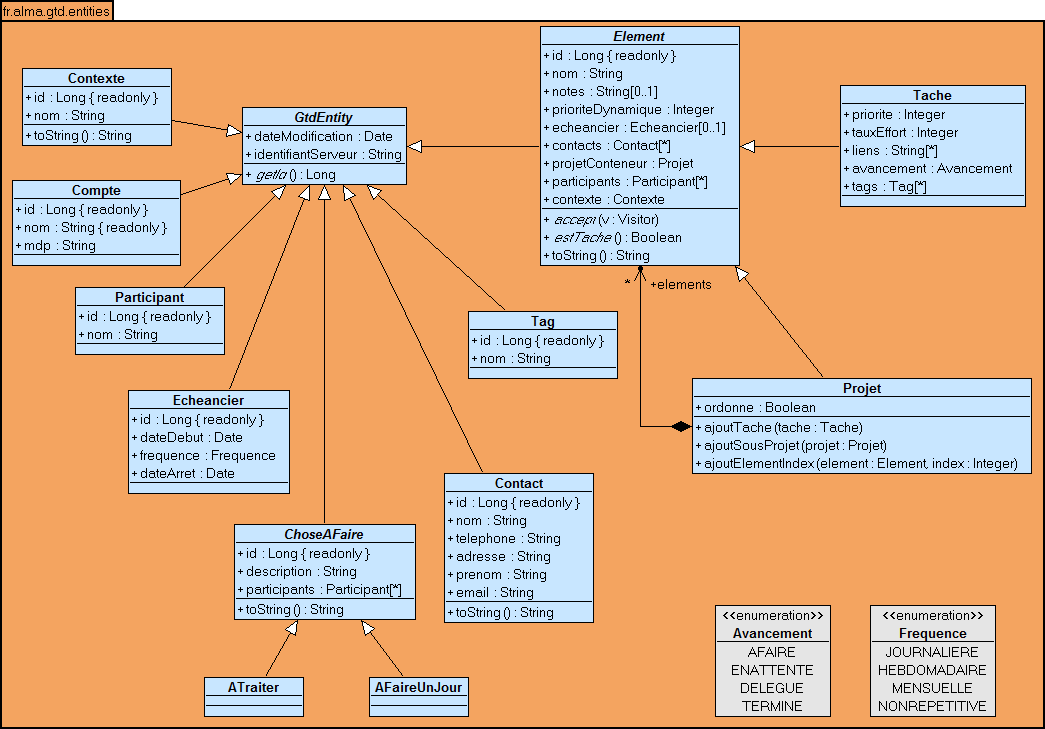
\includegraphics[width=12cm]{diagramme.png}
\caption{Diagramme de classes des entités}
\label{diagclasses}
\end{center}
\end{figure}

Nous obtenons alors le diagramme de classes de la figure~\ref{diagclasses}. 

\subsection{Stratégies de persistance employées}

\subsubsection{Relations entre les entités}
La plupart des relations multi-évaluées entre entités sont des collections d'entités, que l'on peut spécifier sans problème au gestionnaire de persistance, à l'exception des collections de liens que nous avons cité précédemment.
Pour la persistance de ces liens, nous avons employé l'annotation ``\texttt{@CollectionOfElements}'' qui ne provient non pas de JPA, mais du mécanisme de persistance d'Hibernate.
Toutes les relations entre entités sont ici de type ``\texttt{@OneToOne}'', ``\texttt{@ManyToOne}'' ou ``\texttt{@ManyToMany}'', à l'exception de la relation entre un projet et les éléments qu'il contient.
Dans ce cas précis, nous assurons la bidirection de l'association en spécifiant à l'annotation ``\texttt{@OneToMany}'' quel est l'attribut qui correspond dans la classe opposée.
Nous obtenons le code suivant~:
\begin{itemize}
\item dans ``element.java''~:
\begin{lstlisting}
@ManyToOne
protected Projet projetConteneur;
\end{lstlisting}
\item dans ``projet.java''~:
\begin{lstlisting}
 @OneToMany(cascade = CascadeType.ALL, fetch = FetchType.EAGER, mappedBy = "projetConteneur")
private Collection<Element> elements;
\end{lstlisting}
\end{itemize}
Préciser ce ``mapping'' nous permet également d'éviter la création d'une table de correspondance entre les projets et leurs éléments, ce qui optimise la base de données.

\subsubsection{Arbres d'héritages}
Les tâches et les projets sont agencés selon le patron de conception composite~; leur superclasse abstraite devient alors une entité supplémentaire.
Nous avons choisi de représenter cet arbre d'héritage en utilisant la stratégie ``une table par classe fille''\footnote{annotation ``\texttt{@Inheritance(strategy = InheritanceType.JOINED)}''}, qui permet l'accès rapides aux entités projets ou tâches, tout en conservant un accès direct aux propriétés communes entres ces deux types d'entités.
Nous avions pensé à spécialiser les projets en des projets ordonnés et non-ordonnés, mais nous n'avons jamais besoin d'accéder à seulement une des ces deux spécialisations, et la différenciation à partir d'un attribut booléen paraît alors plus adaptée.

En revanche, nous avons choisi de spécialiser les choses à faire en deux sous-classes, car nous n'accédons systématiquement qu'à un seul type de choses à faire.
Nous utilisons dans ce cas la stratégie ``une table pour une hiérarchie de classes''\footnote{annotation ``\texttt{@Inheritance(strategy = InheritanceType.SINGLE\_TABLE)}''}, car il n'y a pas d'attributs supplémentaires dans ces spécialisations.
Nous devons alors spécifier une colonne discrimante à l'aide de l'annotation ``\texttt{@DiscriminatorColumn}'' (dont nous pouvons déclarer le type\footnote{par exemple le type ``\texttt{DiscriminatorType.STRING}''}) pour préciser la spécialisation de l'objet persisté.
Ici, les classes de choses à traiter et de choses à faire un jour sont différenciées respectivement par les annotations ``\texttt{@DiscriminatorValue("A\_TRAITER")}'' et ``\texttt{@Dis\-cri\-mi\-na\-tor\-Value("A\_FAIRE")}''.

\subsubsection{Enumérations}
Les tâches ont quand à elles quatre états possibles, à savoir les tâches à faire, les tâches en attente, les tâches déléguées et les tâches terminées.
Nous avons représenté ces états non pas par des spécialisations de la tâches, ce qui n'apporterait rien du point de vue conceptuel et qui nécessiterait la création d'un nouvel arbre d'héritage, mais par une énumération, ce qui est très bien reconnu par le gestionnaire de persistance.
Même si les requêtes sur un type de tâches précis requiert une clause ``\texttt{WHERE}'', la plupart des requêtes concerne toutes les tâches à la fois.
De la même manière, l'échéancier dispose d'une fréquence de répétition également représentée à l'aide d'une énumération\footnote{annotation ``\texttt{@Enumerated}''}.
Nous précisons au gestionnaire que ces deux énumérations sont enregistrées en tant que chaînes de caractères\footnote{type ``\texttt{EnumType.STRING}''}.

\subsubsection{Gestion des dates}
Afin de déclarer les dates présentes dans l'échéancier, nous avons employé l'annotation ``\texttt{@Temporal}'', qui permet, en plus de signaler qu'il s'agit d'un attribut de date, de spécifier que le type utilisé est ``\texttt{TemporalType.DATE}''.
Les dates sont ainsi correctement persistées dans la base de données.

\section{Création des DAO}
Afin de faciliter la gestion des entités nouvellement créées, nous utilisons le patron de conception DAO\footnote{Data Access Object}.
Ce patron fait la séparation entre le code spécialisé lié aux requêtes faites sur les entités et le code métier.
Pour développer ce patron, nous nous sommes grandement inspiré de l'exemple de code fourni par M.~Thimel, que nous avons ensuite modifié et complété.

\chapter{Conclusion}
Ce projet nous aura permis de mieux comprendre le fonctionnement des mécanismes de persistance tels que le gestionnaire d'entités d'Hibernate, ainsi que de nous familiariser avec les entités JPA, autrement qu'avec les EJB. 

Nous avons également découvert H2, qui est un formidable outil que nous réutiliserons certainement pour d'autres projets (comme par exemple le projet de fin d'études).

\end{document}
